% Template LaTeX document for CSSR4Africa Deliverables
% Adapted from documents prepared by EPFL for the RobotCub project
% and subsequently by the University of Skövde for the DREAM project
%
% DV 28/06/2023

\documentclass{CSSRforAfrica}

\usepackage[titletoc,title]{appendix}
\usepackage[colorlinks, urlcolor=blue, linkcolor=black, citecolor=black]{hyperref}
\usepackage{latexsym}
\usepackage{comment}
\usepackage{multirow}
\usepackage{subcaption}
\usepackage{tabularx}
\usepackage[breakable,skins,most]{tcolorbox} % Consolidated tcolorbox options
\usepackage{tabularx,colortbl}
\usepackage[tikz]{bclogo} % for boxes
\usepackage{ragged2e}
\usepackage{dirtree}
\usepackage{listings}
\usepackage{textcomp}
\usepackage{natbib}
\usepackage{url}
\usepackage{graphicx}
\usepackage{array}
\usepackage{longtable}
\usepackage{algorithm}
\usepackage{algorithmicx}
\usepackage{algpseudocode}
\usepackage{makecell}

%%% for listing %%%%%%%%%%%%%%%%%%%%%%%%%%%%%%
\captionsetup[figure]{format=hang}
\usepackage{xcolor}
\definecolor{codegreen}{rgb}{0,0.6,0}
\definecolor{codegray}{rgb}{0.5,0.5,0.5}
\definecolor{codepurple}{rgb}{0.58,0,0.82}
\definecolor{backcolour}{rgb}{0.95,0.95,0.92}
\definecolor{greenyellow}{rgb}{0.8, 0.7, 0.10} % Example values, adjust as needed

\lstdefinestyle{withoutNumbering}{
	backgroundcolor=\color{backcolour},   
	commentstyle=\color{codegreen},
	keywordstyle=\color{magenta},
	stringstyle=\color{codepurple},
	basicstyle=\ttfamily\small,
	breakatwhitespace=false,         
	breaklines=true,                 
	captionpos=b,                    
	keepspaces=true,                 
	showspaces=false,                
	showstringspaces=false,
	showtabs=false,                  
	tabsize=2
}
%%%%%%%%%%%%%%%%%%%%%%%%%%%%%%%%%%%%%%%%%%%%%%%%%%%
\definecolor{backcolour}{rgb}{0.95,0.95,0.95}
\definecolor{irongray}{HTML}{6D6E71}
\definecolor{LightGray}{gray}{0.9}

\newcommand{\blank}{~\\}
\newcommand{\checkbox}{{~~~~~~~\leavevmode \put(-7,-1.5){  \huge $\Box$  }}}

\begin{document}
\input{epsf}

%%
%% SHOULD NOT NEED TO BE CHANGED BEFORE THIS POINT
%% ------------------------------------------------
%%


\deliverable{D4.2.1}    
\title{D4.2.1 Person Detection and Localization}  

\leadpartner{Carnegie Mellon University Africa} % REPLACE with partner name: Carnegie Mellon University Africa or The University of the Witwatersrand
\partner{}                                      

\revision{1.4}    
\deliverabledate{31/12/2023}  
\submissiondate{21/02/2025} 
\revisiondate{20/06/2025}  
\disseminationlevel{PU}
\responsible{Yohannes Haile}    


%%
%% Create the titlepage
%%

\maketitle
 

\section*{Executive Summary}
%===============================================================
\label{executive_summary}
%%\addcontentsline{toc}{section}{Executive Summary}
Deliverable D4.2.1 focuses on the development of a ROS node that detects and localizes people under various conditions. This deliverable includes the implementation of a ROS node called \\
\texttt{personDetection}, accompanied by a comprehensive report documenting the development process, refinement of requirements, and a detailed specification of the node's functional characteristics. Additionally, it provides a user manual with clear instructions on building and launching the ROS node. The design of the interface covers input, output, and control data, with suitable data structures and code that adhere to the software engineering standards established by the project. The functionality of the \texttt{personDetection} node is thoroughly tested and validated using various test cases, including scenarios with different lighting conditions, occlusions, and varying distances between the robot and the user. The node is also tested on the Pepper robot to confirm its reliability and real-time performance, ensuring it meets the intended objectives effectively.
 
 
\pagebreak
\tableofcontents
\newpage

\section{Introduction}
%===============================================================
This document outlines the development and implementation of a ROS node for person detection and localization. The primary goal of this node is to enhance the interaction capabilities of the Pepper robot, allowing it to identify and track people within its environment, which serves as the behavior controller to initiate interaction as specified in behavior specification. 

The deliverable includes a detailed report documenting the complete software development life cycle for the person detection and localization module. The requirements definition process is thoroughly covered, ensuring that all functional necessities are carefully aligned with the project's objectives. This section also highlights any identified misalignment or challenges that may arise during the development process and how they are addressed. The module design section provides an in-depth description of the person detection localization functionality, covering critical aspects such as input, output, and control data.

The operation of the module is guided by parameters defined in a configuration file, which is structured as a list of key-value pairs in the \texttt{person\_detection\_configuration.json} file. This configuration allows for flexible and scalable customization of the module's behavior to suit various operating conditions and requirements. Furthermore, the document emphasizes the importance of robust design principles to ensure the module's reliability and performance in real-time applications.

\newpage

\section{Requirements Definition}
The person detection and localization module is designed to meet the following requirements, ensuring seamless integration with the Pepper robot and its ROS-based ecosystem. The key requirements for the module are as follows:
\subsection*{Person Detection}
\begin{itemize}
	\item Detect people in the robot’s field of view using an RGB image as input.
	\item Detect and localize all people in the field of view when multiple people are present.
	\item Localize each person by determining their position in the image and drawing bounding boxes.
	\item Identify the centroid coordinates of each bounding box.
	\item Determine the depth (distance from Pepper robot) of all the people detected.
\end{itemize}

\subsection*{Person Labeling and Consistency}
\begin{itemize}
	\item Assign unique labels to each detected person (e.g., ``Person 1").
	\item Maintain consistent labeling of the same person across consecutive image frames, provided the spatial displacement is within a defined tolerance.
	\item Reassign new labels to reappearing persons if not detected for a configurable number of images.
\end{itemize}

\subsection*{Configurable Parameters}
\begin{itemize}
	\item Allow customization through a configuration file (\texttt{person\_detection\_configuration.json})
\end{itemize}

\subsection*{Input/Output Specifications}
\begin{itemize}
	\item \textbf{Input}: RGB-D image from a robot camera or external camera.
	\item \textbf{Output}: Annotated images with bounding boxes and labeled person records published to the \texttt{/personDetection/data} topic.
\end{itemize}

\subsection*{Verbose Mode}
\begin{itemize}
	\item Provide optional diagnostic output and visual debugging through an OpenCV window.
\end{itemize}

\subsection*{Misalignment of the module}
Due to the poor camera present on the robot camera it necessitated the use of external camera. Hence, the depth information provided by the Pepper's camera is low quality hence the depth information (distance of the people from the camera) isn't accurate. In addition, this module doesn't support the simulator. 

\newpage	

\section{Module Specifications}
The person detection module, implemented as a ROS node named personDetection, is designed to detect people within Pepper robot's field of view and determine their location in the image frame of reference. The module provides labeled, color-coded bounding boxes around each detected person and tracks these label across successive images for coherent detection. 

The inputs for this module is an RGB image from the robot's camera or external camera (Intel RealSense D435i), the depth iamge from the robot's depth sensors or an external RGB-D camera (Intel Realsense D435i).

The outputs for this module is annotated RGB image with bounding boxes around detected people and an array of record is published with the following message \texttt{personDetection/data} topic:
\begin{itemize}
	\item Person label representing as number
	\item 3D image coordinates of the bounding box centroid
	\item Width and height of the bounding box
\end{itemize}

\texttt{YOLO} is a deep learning framework optimized for real-time object detection, and when tailored for person detection it accurately identifying human figures in diverse environments. Once persons are detected, the system integrates SORT (Simple Online and Realtime Tracking) for tracking across frames. SORT uses techniques like Kalman filtering and the Hungarian algorithm to maintain consistent identities for each detected individual, even as they move or occlude one another. This combination between YOLO's rapid detection and SORT's efficient tracking provides a robust solution for real-time monitoring for Pepper robot.\cite{yolo}

If verbosemode is set to True in the configuration file, an OpenCV window displays the detected person's bounding box. Each detected person is assigned a unique label. This provides real-time visualization and tracking for person detection. 

A unit test is developed to cover various scenarios, including multiple people, partial occlusion, variable lighting conditions, and label reassignment when the person disappear. The tests are conducted using a driver-stub test platform, which utilizes recorded color and depth images stored in the data folder. Additionally, the unit tests can be executed directly on the physical robot to validate real-world performance.

\newpage

\section{Module Design}

\subsection*{Image Input}
The primary input for the ROS node be the Intel RealSense camera mounted on top of Pepper's head. As an alternative, the Pepper camera can also be used by configuring the camera parameter in the configuration file. However, as noted in section 2 the depth camera has very low quality. The Intel RealSense camera provides both RGB and depth images at various resolutions and frame rates, which can be customized through the launch file parameters. Table \ref{tab:stream_configurations} outlines the available resolution and frame rate configurations for the Intel RealSense camera.

\begin{table}[h!]
	\centering
	\begin{tabular}{|>{\centering\arraybackslash}m{2.5cm}|>{\centering\arraybackslash}m{3cm}|>{\centering\arraybackslash}m{3.0cm}|>{\centering\arraybackslash}m{5cm}|}
		\hline
		\rowcolor{blue!20} % Light blue background color
		\textbf{Format} & \textbf{Resolution} & \textbf{Frame Rate (FPS)} & \textbf{Comment} \\ \hline
		\multirow{6}{*}{Z [16 bits]} & 1280x720 & 6, 15, 30 & \multirow{6}{*}{Depth} \\ \cline{2-3}
		& 848x480 & 6, 15, 30, 60, 90 & \\ \cline{2-3}
		& 640x480 & 6, 15, 30, 60, 90 & \\ \cline{2-3}
		& 640x360 & 6, 15, 30, 60, 90 & \\ \cline{2-3}
		& 480x270 & 6, 15, 30, 60, 90 & \\ \cline{2-3}
		& 424x240 & 6, 15, 30, 60, 90 & \\ \hline
		
		\multirow{9}{*}{YUY2 [16 bits]} & 1920x1080 & 6, 15, 30 & \multirow{9}{*}{\parbox{5cm}{Color Stream from RGB camera \\ (Camera D415 \& D435/D435i)}} \\ \cline{2-3}
		& 1280x720 & 6, 15, 30 & \\ \cline{2-3}
		& 960x540 & 6, 15, 30, 60 & \\ \cline{2-3}
		& 848x480 & 6, 15, 30, 60 & \\ \cline{2-3}
		& 640x480 & 6, 15, 30, 60 & \\ \cline{2-3}
		& 640x360 & 6, 15, 30, 60 & \\ \cline{2-3}
		& 424x240 & 6, 15, 30, 60 & \\ \cline{2-3}
		& 320x240 & 6, 30, 60 & \\ \cline{2-3}
		& 320x180 & 6, 30, 60 & \\ \hline
	\end{tabular}
	\caption{Stream Configurations for Depth and Color for Intel RealSense D435i. See the official datasheet: \href{https://cdrdv2-public.intel.com/841984/Intel-RealSense-D400-Series-Datasheet.pdf}{Intel RealSense D400 Series Datasheet}.}
\label{tab:stream_configurations}
\end{table}

\subsection*{Algorithm}
\subsubsection*{YOLO (You look only Once)}
The YOLO algorithm is an deep learning method for real-time object detection. It uses a single convolutional neural network to predict multiple bounding boxes and class probabilities for each object in the frame. The model divides the image into a grid and makes predictions for each cell simultaneously, allowing it to detect multiple objects quickly and accurately. YOLO’s architecture significantly reduces computation time, making it suitable for real-time applications. During post-processing, overlapping boxes are filtered using non-max suppression to ensure precision and reduce false positives. When employed for person detection specifically, YOLO efficiently isolates human figures in complex environments, enabling fast and reliable identification even in dynamic scenes. In our implementation, we are using the YOLOV8s model, a state-of-the-art variant optimized for enhanced speed and accuracy. YOLOV8s retains the core strengths of the original YOLO framework while offering improvements in efficiency and detection performance. YOLOV8 comes with five variants based on the number of parameter nano(n), small(s), medium(m), large(l), and extralarge(x). We are employing the small(s) variant which is designed for resource-constrained environments and delivers faster inference.

\subsubsection*{SORT (Simple Online and Realtime Tracker)}
The SORT algorithm is a lightweight multi-object tracking method that combines Kalman filtering for motion prediction and the Hungarian algorithm for data association. The process begins with detecting a person using an Intel RealSense camera mounted on Pepper's head. YOLO is employed for head detection, after which the Kalman filter predicts the motion of detected objects in subsequent frames. To associate new detections with existing tracks, SORT utilizes the Hungarian algorithm with Intersection over Union (IoU) as the matching criterion. Once matches are found, the Kalman filter updates its state with the latest information. Tracks that do not find a match are marked as lost and eventually deleted, while new detections initiate new tracks.\cite{SORT}

\begin{algorithm}
	\caption{SORT Algorithm}
	\textbf{Require:} Detected bounding boxes $B_t$ at time $t$, tracked objects $O_{t-1}$ from time $t-1$ \\
	\textbf{Ensure:} Updated object IDs and bounding boxes $O_t$
	\begin{algorithmic}[1]
		\If{$O_{t-1}$ is empty}
		\ForAll{bounding box $b \in B_t$}
		\State \textbf{Register} $b$ as a new object with a unique ID
		\EndFor
		\Else
		\State Predict new positions of tracked objects using the \textbf{Kalman filter}
		\State Compute the cost matrix $D$ using \textbf{Intersection over Union (IoU)} between $B_t$ and predicted objects
		\State Solve the assignment problem using the \textbf{Hungarian algorithm}
		
		\ForAll{matched pairs $(o, b)$}
		\State Update object $o$ with new bounding box $b$
		\State Reset disappearance counter for $o$
		\EndFor
		
		\ForAll{unmatched objects in $O_{t-1}$}
		\State Increment disappearance counter
		\If{counter exceeds threshold}
		\State \textbf{Deregister} the object
		\EndIf
		\EndFor
		
		\ForAll{unmatched bounding boxes in $B_t$}
		\State \textbf{Register} bounding box $b$ as a new object with a unique ID
		\EndFor
		\EndIf
		\State \Return updated objects $O_t$
	\end{algorithmic}
\end{algorithm}

\newpage

Figure \ref{fig: SORT Diagram} illustrates the complete process of SORT tracking.

\begin{figure}[!hbpt]
	\centering
	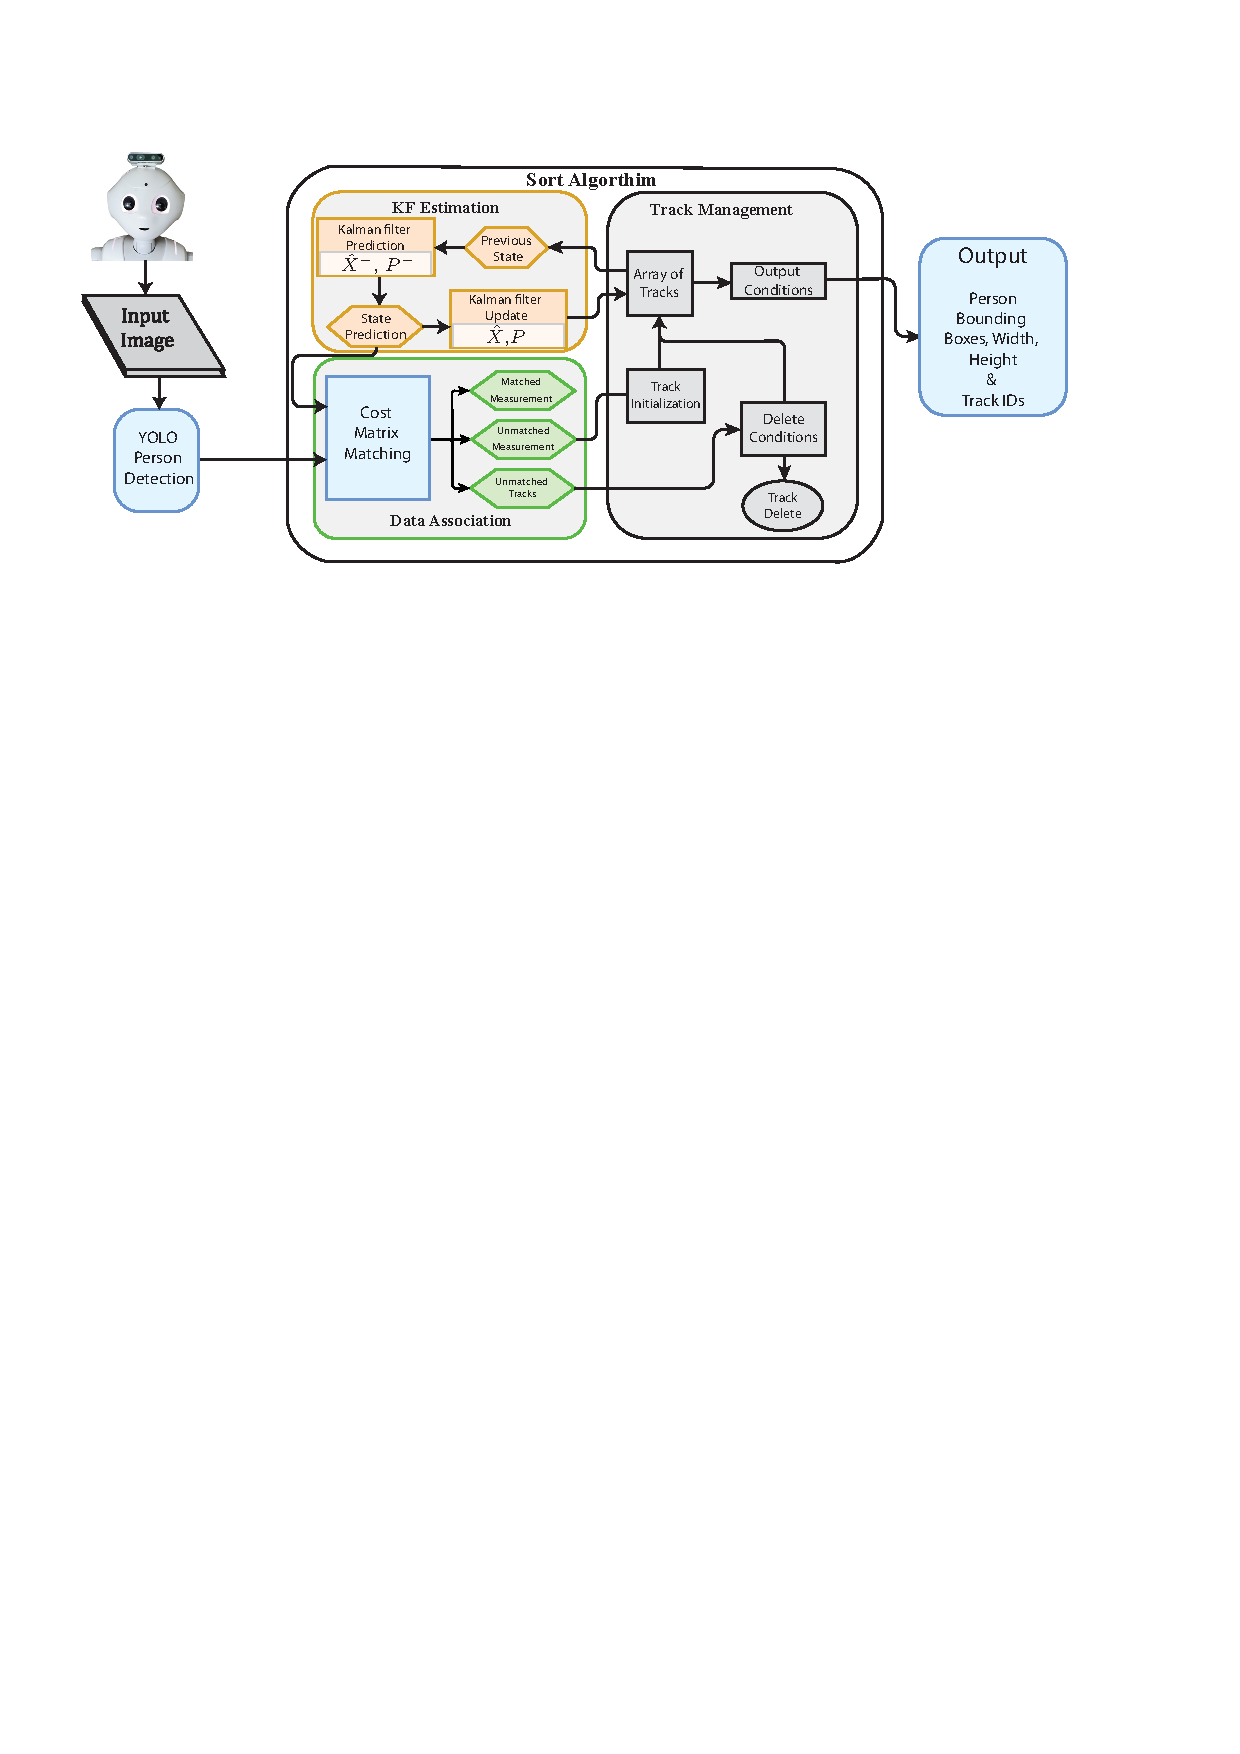
\includegraphics[scale=0.8]{images/SORT_Diagram.pdf}
	\caption{SORT Diagram.}
	\label{fig: SORT Diagram}
\end{figure}

\newpage

\section{Implementation}
\subsection*{File Organization}
The source code for conducting person detection and localization is structured into three primary components: \texttt{person\_detection\_application}, \texttt{person\_detection\_implementation}, and \texttt{person\_detection\_tracking}. The \texttt{person\_detection\_implementation} component encapsulates all the essential functionality required for executing YOLO based person detection. The \texttt{person\_detection\_tracking} component, on the other hand, manages tracking functionality by employing \texttt{SORT} (Simple Online and Realtime Tracking). Additionally, the person detection system is equipped with the capability to process various files critical for testing, such as configuration files, input files, and topic files. Meanwhile, the \texttt{person\_detection\_application} component serves as the entry point, invoking the main functions to run the person detection node and executing the functions defined within \texttt{person\_detection\_implementation}.\\

Figure \ref{fig:person_detection_directory} shows the file structure of the person detection package.

\begin{figure}[h]	
	\renewcommand*\DTstyle{\ttfamily}
	\dirtree{%
		.1 cssr\_system.
		.2 person\_detection.
		.3 config.
		.4 person\_detection\_configuration.json.
		.3 data.
		.4 pepper\_topics.dat.
		.3 launch.
		.4 person\_detection\_launch\_robot.launch.
		.3 models.
		.4 person\_detection\_yolov8s.onnx.
		.3 msg.
		.4 person\_detection\_msg\_file.msg.
		.3 src.
		.4 person\_detection\_application.py.
		.4 person\_detection\_implementation.py.
		.4 person\_detection\_tracking.py.
		.3 person\_detection\_requirements\_x86.txt.
		.3 README.md.
		.2 CSSR4AfricaLogo.svg.
		.2 CMakeLists.txt.
		.2 Package.xml.
	}
	\caption{File structure of the person detection system.}
	\label{fig:person_detection_directory}
\end{figure}

\subsection*{UML Diagram for the Person Detection and Localization Module}
The UML diagram provides a clear structural representation of the Persons Detection and Localization Module, illustrating the relationships between its core components. It highlights inheritance, where PersonDetectionNode serves as the base class, extended by YOLOv8 for specialized person detection. Associations between tracking components such as Sort, and TrackerUtils emphasize how detected people are tracked using Kalman filtering. 

Figure \ref{fig:Person_implementation_UML} show the UML diagram of person\_detection\_implementation.py
\begin{figure}[!hbpt]
	\centering
	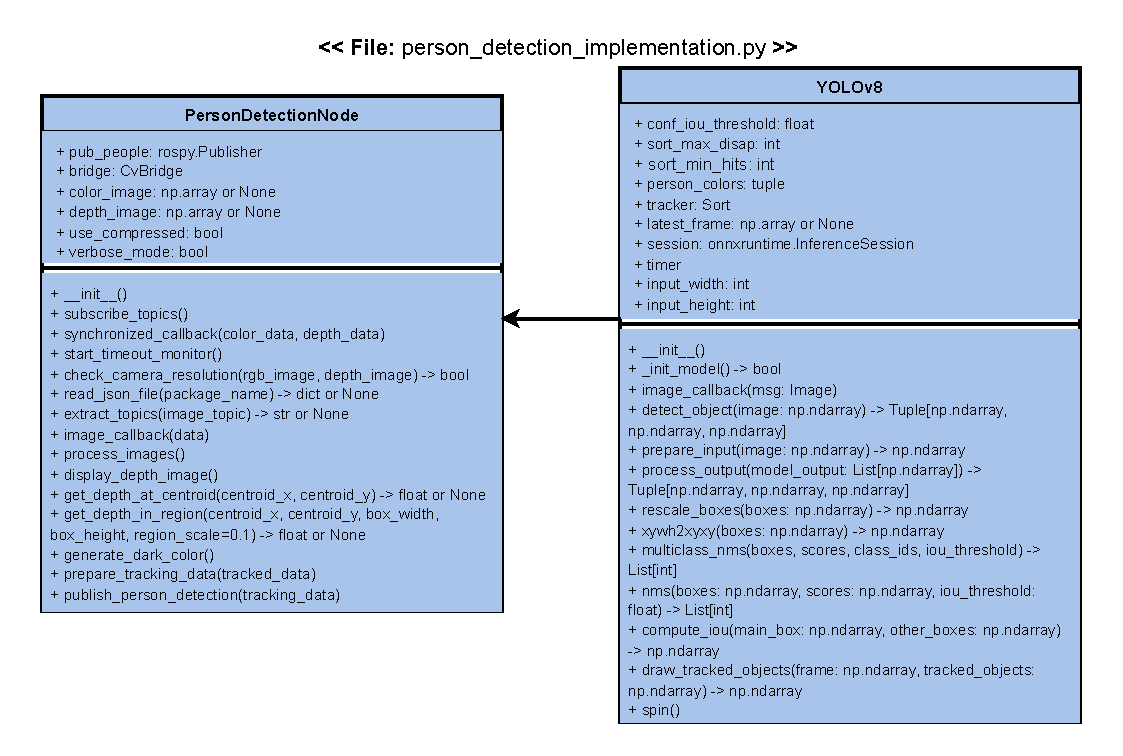
\includegraphics[scale=0.75]{images/Person_implementation_UML.pdf}
	\caption{Person detection implementation UML.}
	\label{fig:Person_implementation_UML}
\end{figure}

Figure \ref{fig:Person_detection_tracking_UML} show the UML diagram of person\_detection\_tracking.py
\begin{figure}[!hbpt]
	\centering
	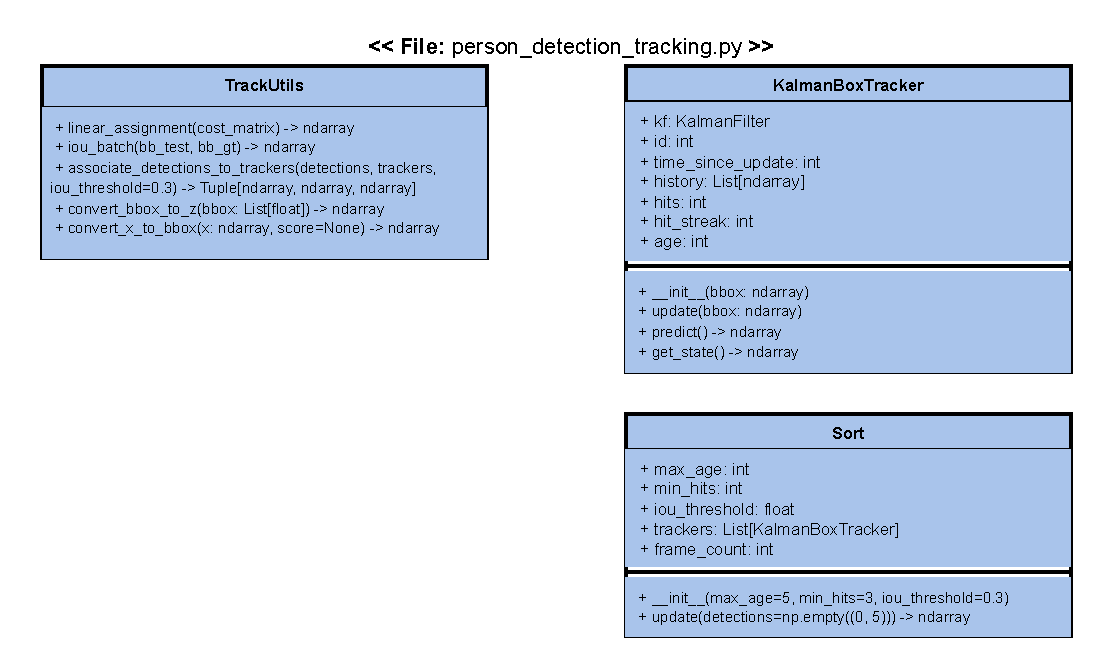
\includegraphics[scale=0.75]{images/Person_Tracking_UML.pdf}
	\caption{Person detection tracking UML.}
	\label{fig:Person_detection_tracking_UML}
\end{figure}

\newpage

\subsection*{Configuration File}
The operation of the person detection node is determined by the contents of the configuration file that contains a list of key-value pairs as shown in Table \ref{tab:person_detection}. 

The configuration file is named \texttt{person\_detection\_configuration.json}. 

\begin{table}[h!]
	\centering
	\begin{tabularx}{\linewidth}{| l | l | X|}
		\hline
		\rowcolor{blue!20} % Light blue background color
		\textbf{Key} & \textbf{Value} & \textbf{Description} \\
		\hline
		{\footnotesize \texttt{useCompressed}}  & {\footnotesize \texttt{true or false}}     & {\small Specifies to use compressed image or raw images.} \\
		\hline
		{\footnotesize \texttt{confidenceThreshold}}  & {\footnotesize \texttt{<number>}}     & {\small Specifies the confidence threshold for the YOLO person detection algorithm.} \\
		\hline
		{\footnotesize \texttt{sortMaxDisappeared}}  & {\footnotesize \texttt{<number>}}     & {\small Specifies the maximum number of frames an object can disappear for SORT tracker before being removed.} \\
		\hline
		{\footnotesize \texttt{sortMinHits}}  & {\footnotesize \texttt{<number>}}     & {\small Specifies the minimum number of consecutive hits required for SORT tracker initialization.} \\
		\hline
		{\footnotesize \texttt{sortIouThreshold}} & {\footnotesize \texttt{<number>}}     & {\small Specifies the Intersection over Union (IoU) threshold for SORT tracker associations.} \\
		\hline
		{\footnotesize \texttt{imageTimeout}} & {\footnotesize \texttt{<number>}}     & {\small Timeout (seconds) for shutting down the node after video ends.} \\
		\hline
		{\footnotesize \texttt{verboseMode}}  & {\footnotesize \texttt{true or false}}     & {\small Specifies whether diagnostic data is to be printed to the terminal and diagnostic images are to be displayed in OpenCV windows.} \\
		\hline
	\end{tabularx}
	\caption{Configuration file key-value pairs for the person detection node.}
\label{tab:person_detection}
\end{table}

\subsection*{Input File}
There is no input file the person detection node.

\subsection*{Output File}
There is no output file the person detection node. The node using OpenCV to display the detected people with bounding boxes and labels.

\subsection*{Models}
The person detection node uses one model for detecting people. The model is stored in the \texttt{models} directory.
\begin{table}[h!]
	\centering
	\begin{tabularx}{\linewidth}{| l | X |}
		\hline
		\rowcolor{blue!20} % Light blue background color
		\textbf{Model} & \textbf{Description} \\
		\hline
		{\footnotesize \texttt{person\_detection\_yolov8s.onnx} }  & {\footnotesize YOLO-based person detection model.} \\
		\hline
	\end{tabularx}
	\caption{Models used by the person detection node.}
\end{table}

\subsection*{Topics File} 
For the test, a selected list of the topics for the robot is stored in the topics file. The topic files are 
written in the .dat file format. The data file is written in key-value pairs where the key is the camera 
and the value is the topic. The topics file for the robot is named \texttt{pepper\_topics.dat}.

\subsection*{Launch File}
The launch file \texttt{person\_detection\_launch\_robot.launch} is designed to initialize either Pepper's front camera or the Intel RealSense camera based on the specified configuration. It declares several parameters that can be customized to match your network settings and camera choice:
\begin{itemize}
	\setlength\itemsep{0em}
	\item \texttt{pepper\_robot\_ip}: specifies the IP address of the Pepper robot (default: \texttt{172.29.111.230}).
	\item \texttt{pepper\_robot\_port}: specifies the communication port for Pepper (default: \texttt{9559}).
	\item \texttt{roscore\_ip}: IP address of the ROS master (default: \texttt{127.0.0.1})
	\item \texttt{network\_interface}: specifies the network interface name (default: \texttt{wlp0s20f3}).
	\item \texttt{namespace}: sets the ROS namespace for the naoqi driver (default: \texttt{naoqi\_driver}).
	\item \texttt{camera}: selects the camera source; set to \texttt{pepper} for Pepper's front camera or \texttt{realsense} for the Intel RealSense camera (default: \texttt{realsense}).
\end{itemize}

The file sets the parameter \texttt{/personDetection/camera} to the chosen camera and conditionally launches the corresponding nodes. If the \texttt{camera} parameter is set to \texttt{pepper}, the launch file starts the \texttt{naoqi\_driver} node using the provided IP, port, network interface, and namespace. Conversely, if \texttt{camera} is set to \texttt{realsense}, it includes the RealSense camera launch file with specified parameters for image resolution, frame rate, and depth alignment. Users can adjust these default values to suit their specific hardware configurations.

\subsection*{Topics Subscribed}
The person detection node subscribes to the  topics shown in Table \ref{tab:topics_subscribed}.
\begin{table}[!h]
	\centering
	{\fontsize{7.0}{9.0}\selectfont % <- apply inside the table
		\begin{tabularx}{\linewidth}{| l | l | X |}
			\hline
			\rowcolor{blue!20}
			\textbf{Camera} & \textbf{Topic Name} & \textbf{Message Type} \\
			\hline
			\texttt{RealSenseCameraRGB} & \texttt{/camera/color/image\_raw} & \texttt{sensor\_msgs/Image} \\
			\hline
			\makecell[l]{\texttt{RealSenseCameraRGB} \\ (Compressed)} & \texttt{/camera/color/image\_raw/compressed} & \texttt{sensor\_msgs/CompressedImage} \\
			\hline
			\texttt{RealSenseCameraDepth} & \texttt{/camera/aligned\_depth\_to\_color/image\_raw} & \texttt{sensor\_msgs/Image} \\
			\hline
			\makecell[l]{\texttt{RealSenseCameraDepth} \\ (Compressed)} & \texttt{/camera/aligned\_depth\_to\_color/image\_raw/compressed} & \texttt{sensor\_msgs/CompressedImage} \\
			\hline
			\texttt{PepperFrontCamera} & \texttt{/naoqi\_driver/camera/front/image\_raw} & \texttt{sensor\_msgs/Image} \\
			\hline
			\texttt{PepperDepthCamera} & \texttt{/naoqi\_driver/camera/depth/image\_raw} & \texttt{sensor\_msgs/Image} \\
			\hline
		\end{tabularx}
	}
	\caption{Topics subscribed by the person detection node.}
\label{tab:topics_subscribed}
\end{table}

\newpage

\subsection*{Topics Published}
The person detection node publishes the  topics shown in Table \ref{tab:topics_published}.
\begin{table}[!h]
	\centering
	\begin{tabularx}{\linewidth}{| l | l | X |}
		\hline
		\rowcolor{blue!20} % Light blue background color
		\textbf{Topic Name} & \textbf{Message Type} & \textbf{Description} \\
		\hline
		{\footnotesize \texttt{/personDetection/data} }  & {\footnotesize \texttt{personDetection/msg\_file}} & {\footnotesize \texttt{An array of records containing person labels, 3D image coordinates of the bounding box, and width and height of the bounding box}} \\
		\hline
	\end{tabularx}
	\caption{Topics published by the person detection node.}
\label{tab:topics_published}
\end{table}

\newpage

\section{Running the Person Detection Node}
To run the person detection node, the user must first install the necessary software packages as outlined in 
\href{https://cssr4africa.github.io/deliverables/CSSR4Africa_Deliverable_D3.3.pdf}{Deliverable 3.3}. The required packages
are listed in the {\scriptsize{\texttt{person\_detection\_requirements.txt}}} file. The user can follow the README file in the person detection
package to install the required packages. Referring to the implementation section of this deliverable report, the user must 
set the configuration file to the desired parameters. Using the key-value pair, the user can set the camera, algorithm, 
confidence threshold, and other parameters. The user can then run the person detection node by executing the following 
command in the terminal:

\begin{lstlisting}[style=withoutNumbering, language=bash]
	# Launch either Pepper Camera or RealSense Camera from the launch file 
	$ roslaunch cssr_system person_detection_launch_robot.launch camera:=pepper
	# or
	$ roslaunch cssr_system person_detection_launch_robot.launch camera:=realsense
\end{lstlisting}

\begin{lstlisting}[style=withoutNumbering, language=bash]
	# Activate the virtual environment:
	source cssr4africa_face_person_detection_env/bin/activate
\end{lstlisting}

\begin{lstlisting}[style=withoutNumbering, language=bash]
	# Run the person detection node
	$ rosrun cssr_system person_detection_application.py
\end{lstlisting}

If the user has set the verboseMode to True in the configuration file, the person detection node displays the detected people with bounding boxes and labels in an OpenCV window.

\newpage
\section{Unit Test}
The unit test is designed to validate the person detection node's functionality under various scenarios, including multiple people, occlusions, and varying lighting conditions. 
The test can be performed using a driver-stub test platform, which utilizes recorded color and depth images stored in the data folder as a rosbag file. The unit test can also 
be executed directly on the physical robot to validate real-world performance. 

The person detection unit test file structure is as shown in Figure \ref{fig:person_detection_unit_test}

\begin{figure}[h]	
	\renewcommand*\DTstyle{\ttfamily}
	\dirtree{%
		.1 unit\_test.
		.2 person\_detection\_test.
		.3 config.
		.4 person\_detection\_test\_configuration.json.
		.3 data.
		.4 person\_detection\_test\_input\_single\_person.bag.
		.4 person\_detection\_test\_input\_multiple\_people.bag.
		.4 person\_detection\_test\_input\_lighting\_1.bag.
		.4 person\_detection\_test\_input\_lighting\_2.bag.
		.3 launch.
		.4 person\_detection\_test\_launch\_robot.launch.
		.4 person\_detection\_test\_launch\_test\_harness.launch.
		.3 msg.
		.4 person\_detection\_test\_msg\_file.msg.
		.3 src.
		.4 person\_detection\_test\_application.py.
		.4 person\_detection\_test\_implementation.py.
		.3 README.md.
		.2 CSSR4AfricaLogo.svg.
		.2 CMakeLists.txt.
		.2 Package.xml.
	}
	\caption{File structure of the person detection unit test.}
	\label{fig:person_detection_unit_test}
\end{figure}

The test cases for the person detection node that are going to be evaluated are as shown in Table \ref{tab:person_detection_tests}.
\newpage

\begin{longtable}{| l | p{10cm} |}
	\hline
	\rowcolor{blue!20} % Light blue background color
	\textbf{Test Case} & \textbf{Description} \\
	\hline
	\endfirsthead
	
	% Continuation header for the next pages
	\hline
	\rowcolor{blue!20} 
	\textbf{Test Case} & \textbf{Description} \\
	\hline
	\endhead
	
	% Table content
	\text{Single Person Detection} & Verify the person detection node's ability to detect and localize a single person in the image frame, as well as evaluate the distance at which the person is detected. \\
	\hline
	\text{Multiple Person Detection} & Validate the person detection node's capability to detect and localize multiple people in the image frame. \\
	\hline
	\text{Person Tracking} & Test the person detection node's tracking functionality by tracking a person across multiple frames. \\
	\hline
	\text{Occlusion Handling} & Evaluate the person detection node's performance in handling partial occlusions of person. \\
	\hline
%%	\newpage
	\text{Lighting Conditions} & Test the person detection node's robustness under varying lighting conditions. \\
	\hline
	\caption{Test cases for person detection node evaluation.}
	\label{tab:person_detection_tests}
\end{longtable}

\subsection*{Configuration File}
The configuration file for the person detection unit test is named \\
\texttt{person\_detection\_test\_configuration.json} and contains the  key-value pairs shown in Table \ref{tab:person_detection_key_value_pairs}.

\begin{table}[h!]
	\centering
	\renewcommand{\arraystretch}{1.2} % Increase row height for better readability
	\begin{tabularx}{\linewidth}{|p{3.5cm}|p{4cm}|X|}
		\hline
		\rowcolor{blue!20} % Light blue background color
		\textbf{Key} & \textbf{Value} & \textbf{Description} \\
		\hline
		\texttt{algorithm}      & \texttt{sixdrep or mediapipe} & {\small Specifies the algorithm used for face detection and head pose estimation.} \\
		\hline
		\texttt{useCompressed}   & \texttt{true or false}       & {\small Specifies to use compressed image or raw images.} \\
		\hline
		\texttt{saveVideo}       & \texttt{true or false}       & {\small Specifies whether to save the output video of the test.} \\
		\hline
		\texttt{saveImage}       & \texttt{true or false}       & {\small Specifies whether to save individual image frames from the test.} \\
		\hline
		\texttt{videoDuration}   & \texttt{<number>}            & {\small Specifies the duration (in seconds) for which the video is saved.} \\
		\hline
		\texttt{imageInterval}   & \texttt{<number>}            & {\small Specifies the time interval (in seconds) at which images are captured and saved.} \\
		\hline
		\texttt{recordingDelay}  & \texttt{<number>}            & {\small Delay (seconds) before recording starts.} \\
		\hline
		\texttt{maxFrameBuffer}  & \texttt{<number>}            & {\small Maximum number of frames to store in buffer.} \\
		\hline
		\texttt{verboseMode}     & \texttt{true or false}       & {\small Specifies whether detailed logs and diagnostic images are displayed during execution.} \\
		\hline
	\end{tabularx}
	\caption{Configuration file key-value pairs for the person detection test.}
	\label{tab:person_detection_key_value_pairs}
\end{table}

\noindent \textbf{Note:} Valid values for \texttt{bag\_file} include:  
\texttt{single\_person}, \texttt{multiple\_people}, \texttt{lighting\_1}, \texttt{lighting\_2}.

\subsection*{Input File}
The node takes recorded RGB and depth video saved as rosbag file as an input. 

\subsection*{Output File}
The node has the option to save a recorded video and/or image with the bounding box and mutual gaze determined.

\subsection*{Launch File}
The launch file \texttt{person\_detection\_test\_launch\_robot.launch} is designed to support testing the person detection node with various input sources: a live feed from Pepper’s front camera, the Intel RealSense camera, or a recorded rosbag video. It provides several configurable arguments to customize the test environment:

\begin{itemize}
	\setlength\itemsep{0em}
	\item \texttt{camera}: selects the camera input source; set to \texttt{pepper} for Pepper's camera, \texttt{realsense} for the RealSense camera, or \texttt{video} to use a recorded rosbag (default: \texttt{video}).
	\item \texttt{bag\_file}: specifies which bag file to play; only used when \texttt{camera=video} \\
	 (default: \texttt{single\_person}).
	\item \texttt{robot\_ip}: IP address of the Pepper robot (default: \texttt{172.29.111.230}).
	\item \texttt{roscore\_ip}: IP address of the ROS master (default: \texttt{127.0.0.1}).
	\item \texttt{robot\_port}: communication port for the Pepper robot (default: \texttt{9559}).
	\item \texttt{network\_interface}: name of the network interface for ROS communication (default: \texttt{wlp0s20f3}).
	\item \texttt{namespace}: ROS namespace for the naoqi driver (default: \texttt{naoqi\_driver}).
\end{itemize}

Depending on the selected input method, the launch file performs the following:

\begin{itemize}
	\item If \texttt{camera} is set to \texttt{realsense}, it launches the RealSense camera driver with pre-configured resolution and frame rate settings.
	\item If \texttt{camera} is set to \texttt{pepper}, it launches the \texttt{naoqi\_driver} node to stream Pepper’s camera data.
	\item If \texttt{camera} is set to \texttt{video}, it plays a specified bag file from the \texttt{unit\_test} package in a loop.
\end{itemize}

This setup allows flexible testing of the face detection node using live or recorded data sources with consistent parameters across different hardware.\\

The launch file \texttt{person\_detection\_test\_launch\_test\_harness.launch} launches the person\_detection node and person\_detection\_test node that run the unit test based on configuration file in the person\_detection\_test.

\newpage

\subsection*{Topics Subscribed}
The person detection test node subscribes to the  topics shown in Table \ref{tab:topics}.

\begin{table}[!h]
	\centering
	{\fontsize{9.0}{12.0}\selectfont % <- apply inside the table
		\begin{tabularx}{\linewidth}{| l | l | X |}
			\hline
			\rowcolor{blue!20}
			\textbf{Camera} & \textbf{Topic Name} & \textbf{Message Type} \\
			\hline
			\texttt{RealSenseCameraRGB} & \texttt{/camera/color/image\_raw} & \texttt{sensor\_msgs/Image} \\
			\hline
			\texttt{RealSenseCameraDepth} & \texttt{/camera/aligned\_depth\_to\_color/image\_raw} & \texttt{sensor\_msgs/Image} \\
			\hline
			\texttt{PepperFrontCamera} & \texttt{/naoqi\_driver/camera/front/image\_raw} & \texttt{sensor\_msgs/Image} \\
			\hline
			\texttt{PepperDepthCamera} & \texttt{/naoqi\_driver/camera/depth/image\_raw} & \texttt{sensor\_msgs/Image} \\
			\hline
		\end{tabularx}
	}
	\caption{Topics subscribed by the person detection test node.}
\label{tab:topics}.
\end{table}

In addition it subscribes to \texttt{/personDetection/data} to draw the bounding box and save the video in the data folder. 

\subsection*{Running Person Detection and Localization Unit Test}
The user can execute the following commands in the terminal to run the unit test for person detection node. 

\begin{lstlisting}[style=withoutNumbering, language=bash]
	# Launch unit test for person_detection by setting the camera to realsense, pepper or video.
	$ roslaunch unit_test person_detection_test_launch_robot.launch camera:=realsense
	# or
	$ roslaunch unit_test person_detection_test_launch_robot.launch camera:=pepper
	# or 
	$ roslaunch unit_test person_detection_test_launch_robot.launch camera:=video
	
\end{lstlisting}

\begin{lstlisting}[style=withoutNumbering, language=bash]
	# Activate the virtual environment:
	source cssr4africa_face_person_detection_env/bin/activate
\end{lstlisting}

\begin{lstlisting}[style=withoutNumbering, language=bash]
	# Run the person detection node
	$ roslaunch unit_test person_detection_test_launch_robot.launch
\end{lstlisting}

The user should validate the node's performance by visually inspecting the images displayed through OpenCV.

\newpage
\bibliographystyle{unsrt}
%================================================================
\bibliography{cognitive_systems.bib}                                     % REPLACE with correct filename
\addcontentsline{toc}{section}{References}

\pagebreak
\section*{Principal Contributors}
%===============================================================
\label{contributors}
\addcontentsline{toc}{section}{Principal Contributors}
The main authors of this deliverable are as follows (in alphabetical order).
\blank
~
\blank
Yohannes Haile, Carnegie Mellon University Africa.\\    % REPLACE with correct name and affiliation
David Vernon, Carnegie Mellon University Africa. \\                                                                           % REMOVE
 

  
\newpage
\section*{Document History}
%================================================================
\addcontentsline{toc}{section}{Document History}
\label{document_history}

\begin{description}
\item [Version 1.0]~\\
First draft.\\
Natasha Mutangana.\\
10 January 2024.

\item [Version 1.1]~\\
Complete rewrite of the deliverable.\\
Yohannes Haile. \\   
21 February 2025.   

\item [Version 1.2]~\\
Changed the notation in Figure 1.\\
Changed the file structure tree in Figure 2.\\
Updated the UML diagram on Figure 3. \\
Updated the configuration Table 2.\\
Updated the file structure in the person\_detection in Figure 3.\\
Updated the file structure in the person\_detection\_test in Figure 6.\\
Updated the Topics subscribed in Table 4. \\
Added width and height of the bounding box. \\
Updated the launch file for person\_detection(Page 13).\\
Removed speaker option from the configuration file Table 7. \\
Updated the name of the rosbag files to use (Page 20).\\
Added width and height in the message field for the msg\_file for the person\_detection.\\
Added input file, output file, running the unit test launch file and Topics subscribed for the unit test.\\
Removed future tense in the report.\\
Yohannes Haile. \\                                    
29 April 2025.  

\item [Version 1.3]~\\
Fixed typos and added explicit references to tables.\\
David Vernon. \\   
16 June 2025.  

\item [Version 1.4]~\\
Added explicit references to the figures.\\
Yohannes Haile.\\
20 June 2025.

 
\end{description}

\end{document}

